\documentclass[a4paper,12pt]{article}
\usepackage{graphicx}

\usepackage{epstopdf}
\usepackage{gensymb}
\usepackage{float}
\usepackage{amssymb}
\usepackage{amsmath}
\usepackage{mathtools}
\usepackage{braket}
\usepackage{setspace}
\usepackage{tabularx}
\usepackage{longtable}

\usepackage{lipsum}
\usepackage{booktabs}
\usepackage{array}
\newcolumntype{R}{>{\raggedleft\arraybackslash}p{6cm}}

\title{Teknisk Dokumentation}
%% Definitioner för LIPS-dokument

\usepackage[swedish]{babel}
\usepackage[utf8]{inputenc}
\usepackage[T1]{fontenc}
\usepackage{times}
\usepackage{ifthen}
\usepackage[labelfont=it]{caption}

\usepackage[margin=25mm]{geometry}

\def\arraystretch{1.6}

\usepackage{fancyhdr}
\pagestyle{fancy}
\lhead{}
\chead{\LIPSprojekttitel}
\rhead{\LIPSdatum}
\lfoot{\LIPSkursnamn \\ \LIPSdokumentansvarig}
\rfoot{\LIPSprojektgrupp \\ \LIPSgruppepost}

\setlength{\parindent}{0pt}
\setlength{\parskip}{1ex plus 0.5ex minus 0.2ex}


\newcommand{\twodigit}[1]{\ifthenelse{#1<10}{0}{}{#1}}
\newcommand{\dagensdatum}{\number\year-\twodigit{\number\month}-\twodigit{\number\day}}

%% ------------------------------------------
% NYBILD
% Skapar centrerad bild med caption
%   
% #1: Filens url relativt '/bilder/'
% #2:  Caption
% #3: Label
% #4: Skalning i förhållande till textwidth
%% ------------------------------------------
\newcommand{\nyBild}[4] 
{\begin{figure}[H]
  \centering
 \emph{\includegraphics[angle=0,width=#4\textwidth]{bilder/#1}}
  \caption{\emph{#2}}
  \label{fig:#3}
\end{figure}}

%%  Redefinitions of commands containing @
\makeatletter
\makeatother

\newcommand{\LIPStitelsida}{%
{\ }\vspace{45mm}
\begin{center}
  \textbf{\Huge {\sffamily \LIPSdokumenttyp}}
\end{center}
\begin{center}
  {\Large \LIPSredaktor}
\end{center}
%\begin{center}
%  {\Large Version \LIPSversion}
%\end{center}
\vspace{60mm}
%\begin{center}
%  {\large Status}\\[1.5ex]
%  \begin{tabular}{|*{3}{p{40mm}|}}
%    \hline
%    Granskad & \LIPSgranskare & \LIPSgranskatdatum \\
%    \hline
%    Godkänd & \LIPSgodkannare & \LIPSgodkantdatum \\
%    \hline
%  \end{tabular}
%\end{center}
\newpage
}


\newenvironment{LIPSprojektidentitet}{%
{\ }\vspace{45mm}
\begin{center}
  {\Large PROJEKTIDENTITET}\\[0.5ex]
  {\small
  \LIPSprojektgrupp, \LIPSartaltermin, \LIPSprojekttitel\\
  Tekniska högskolan vid Linköpings universitet, ISY
  }
\end{center}
\begin{center}
  \begin{tabular}{|l|p{45mm}|p{25mm}|l|}
    \hline
    \textbf{Namn} & \textbf{Ansvar} & \textbf{Telefon} & \textbf{E-post} \\
    \hline
}
{
    \hline
  \end{tabular}
\end{center}
\begin{center}
  {\small
    \textbf{E-postlista för hela gruppen}: \LIPSgruppepost\\
    \textbf{Kontaktperson hos kund}: \LIPSkundkontakt\\
    \textbf{Kursansvarig}: \LIPSkursansvarig\\
    \textbf{Handledare}: \LIPShandledare\\
  }
\end{center}
\newpage
}
\newcommand{\LIPSgruppmedlem}[4]{\hline {#1} & {#2} & {#3} & {#4} \\}



\newenvironment{LIPSdokumenthistorik}{%
\begin{center}
  Dokumenthistorik\\[1ex]
  \begin{small}
    \begin{tabular}{|l|l|p{60mm}|l|l|}
      \hline
      \textbf{Version} & \textbf{Datum} & \textbf{Utförda förändringar} & \textbf{Utförda av} & \textbf{Granskad} \\
      }%
    {%
      \hline
    \end{tabular}
  \end{small}
\end{center}
}
\newcommand{\LIPSversionsinfo}[5]{\hline {#1} & {#2} & {#3} & {#4} & {#5} \\}



\newenvironment{packed_itemize}{
\begin{itemize}
	\setlength{\itemsep}{1pt}
    \setlength{\parskip}{0pt}
    \setlength{\parsep}{0pt}
}{\end{itemize}}

\newenvironment{packed_enumerate}{
\begin{enumerate}
	\setlength{\itemsep}{1pt}
    \setlength{\parskip}{0pt}
    \setlength{\parsep}{0pt}
}{\end{enumerate}}





%%% Local Variables: 
%%% mode: latex
%%% TeX-master: "kravspec_mall"
%%% End:

\usepackage{sectsty}
\allsectionsfont{\sffamily}

\frenchspacing

\renewcommand{\thepage}{\roman{page}}

\newcommand{\LIPSartaltermin}{VT14}
\newcommand{\LIPSkursnamn}{TSEA56 Elektronik kandidatprojekt}

\newcommand{\LIPSprojekttitel}{Lagerrobot}

\newcommand{\LIPSprojektgrupp}{Grupp 1}
\newcommand{\LIPSgruppepost}{tsea56-2014-grupp-1@googlegroups.com}
\newcommand{\LIPSdokumentansvarig}{LIPS Användarmanual}

\newcommand{\LIPSkund}{ISY, Linköpings universitet, 581\,83 Linköping}
\newcommand{\LIPSkundkontakt}{Tomas Svensson, 013-28 13 68, tomass@isy.liu.se}
\newcommand{\LIPSkursansvarig}{Tomas Svensson, 013-28 13 68, 3B:528, tomass@isy.liu.se}
\newcommand{\LIPShandledare}{Anders Nilsson, 3B:512, 013-28 26 35, anders.p.nilsson@liu.se}


\newcommand{\LIPSdokumenttyp}{Användarmanual}
\newcommand{\LIPSredaktor}{Lucas Nilsson}
\newcommand{\LIPSversion}{1.0}
\newcommand{\LIPSdatum}{\dagensdatum}

\newcommand{\LIPSgranskare}{}
\newcommand{\LIPSgranskatdatum}{}
\newcommand{\LIPSgodkannare}{}
\newcommand{\LIPSgodkantdatum}{}

\setlength{\parskip}{\baselineskip}%
\setlength{\parindent}{0pt}%

\begin{document}

\LIPStitelsida

%% Argument till \LIPSgruppmedlem: namn, roll i gruppen, telefonnummer, epost
\begin{LIPSprojektidentitet}
  \LIPSgruppmedlem{Karl Linderhed}{Projektledare (PL)}{073-679 59 59}{karli315@student.liu.se}
  \LIPSgruppmedlem{Patrik Nyberg}{Dokumentansvarig (DOK)}{073 -049 59 90}{patny205@student.liu.se}
  \LIPSgruppmedlem{Johan Lind}{}{070-897 58 24}{johli887@student.liu.se}
  \LIPSgruppmedlem{Erik Nybom}{}{070-022 47 85}{eriny778@student.liu.se}
  \LIPSgruppmedlem{Andreas Runfalk}{}{070-564 23 79}{andru411@student.liu.se}
  \LIPSgruppmedlem{Philip Nilsson}{}{073-528 48 86}{phini326@student.liu.se}
  \LIPSgruppmedlem{Lucas Nilsson}{}{073-059 42 94}{lucni395@student.liu.se}
\end{LIPSprojektidentitet}


\renewcommand*\contentsname{Innehåll}
\begin{spacing}{0.5}
\tableofcontents{}
\end{spacing}
\newpage

%% Argument till \LIPSversionsinfo: versionsnummer, datum, ändringar, utfört av, granskat av
%\addcontentsline{toc}{section}{Dokumenthistorik}
\begin{LIPSdokumenthistorik}
  \LIPSversionsinfo{1.0}{}{}{}{}
\end{LIPSdokumenthistorik}
\newpage

\renewcommand{\thepage}{\arabic{page}}
\setcounter{page}{1}

\section{Allmänt}
Produkten är en lagerrobot med uppgiften att i en lagermiljö kunna bli beordrad att förflytta föremål mellan lagerplatser. Roboten är konstruerad att kunna följa svart linje på marken och stanna vid utmarkerade platser för att hämta eller lämna föremål. Användaren kan välja att kontrollera roboten manuellt eller låta den agera autonomt.

\section{Krav på omgivning}
Roboten är designad för att kunna manövrera sig fram längs med en linje vars luminans är betydligt mindre än underlagets. Denna mörka linje bör vara mellan 14-18 mm bred. Upplockningsstationer indikeras med en annan linje på cirka 10 cm vinkelrätt ut från körbanan. Banan är en sluten slinga och får endast korsas i en rät vinkel. Kurvor i körbanan ska ha en radie på minst 25cm. 

Föremål som ska plockas upp har lämpligen liknande dimensioner som en jengakloss och en maxvikt på 200g. Dess placering i förhållande till linjen bör vara inom armens räckvidd men inte heller för nära roboten. Mer om banans utformning i bilaga \ref{banspecifikation}.  

%
%----------------------------------------
%

\section{Användning av roboten}
\begin{figure}[H]
	\centering
	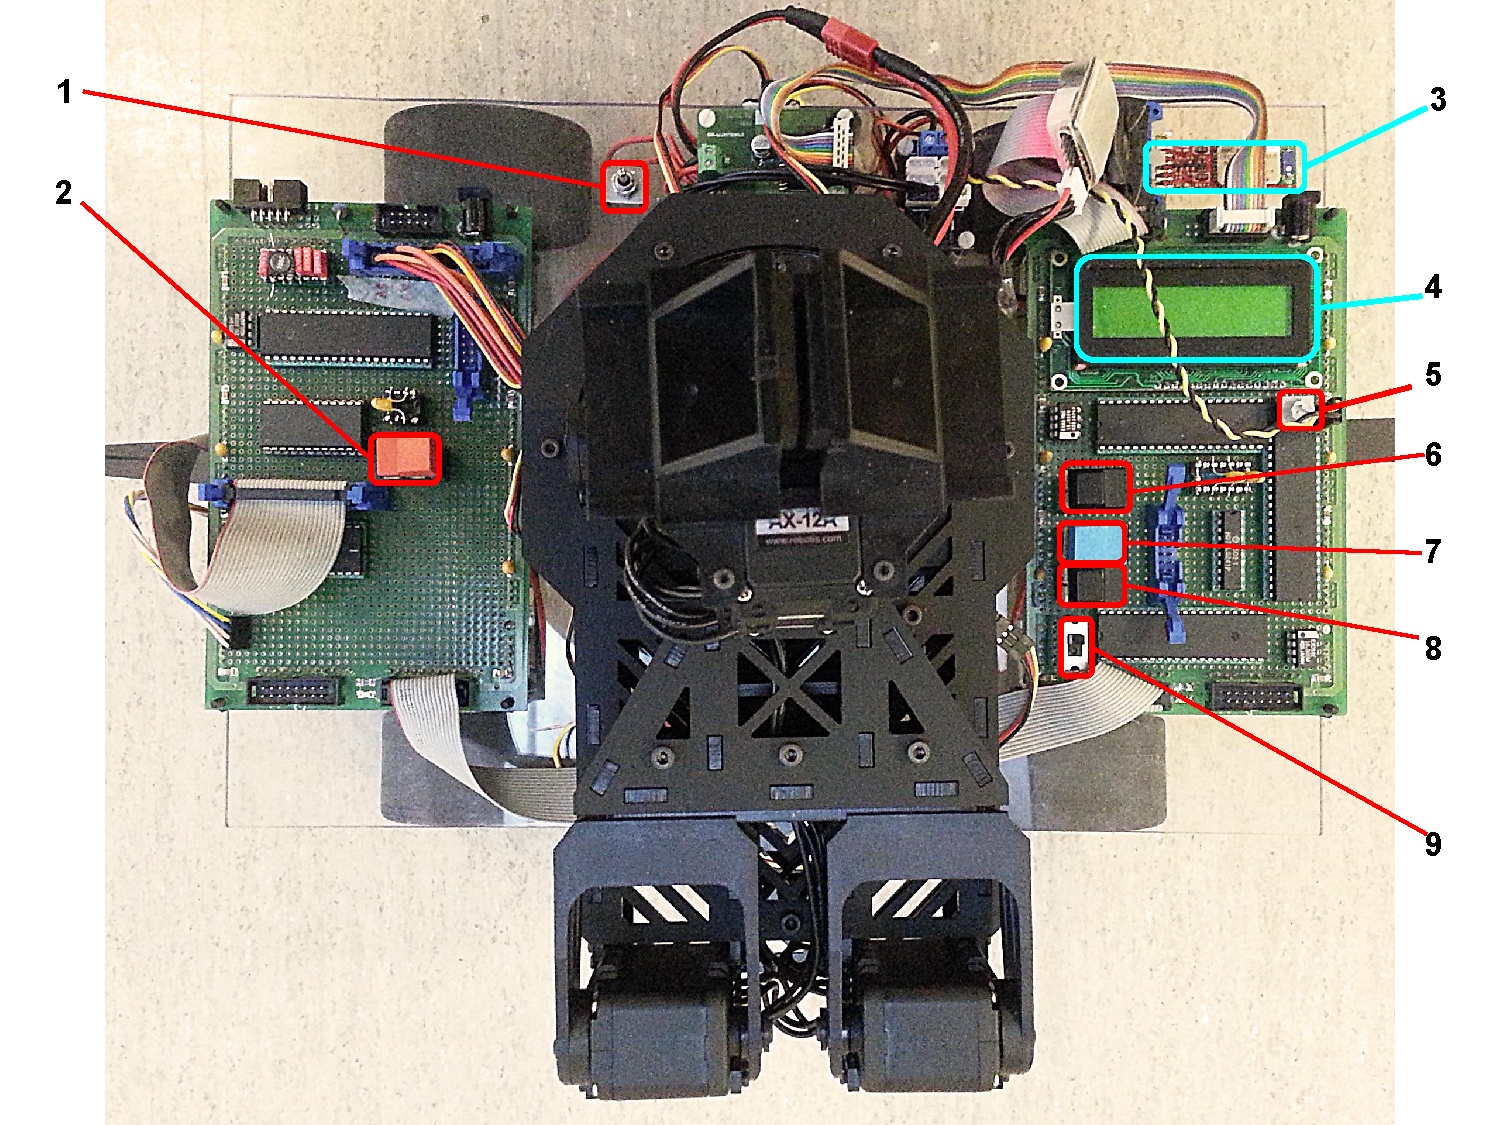
\includegraphics[width=1.0\textwidth]{oversikt_handledning.pdf}
	\caption{Roboten sett ovanifrån med knappar, display och blåtandsenhet markerad och numrerad}
	\label{fig:robot_oversikt}
\end{figure}

I figur \ref{fig:robot_oversikt} är komponenter som är behövliga vid användning av roboten numrerade, nedan kommer dessa refereras till i texten med knappens siffra, till exempel refererar texten till LCD-skärmen med (4).

Roboten använder ett batteri av typen LI-PO TIGER Power Atomic-Platinum 11.1V 2200mAh. Läs igenom all säkerhetsdokumentation och varningar innan denna kopplas på, se till att det är fulladdat och i skick att användas. Se till att alla kablar på roboten är inkopplade och att de inte är i vägen för sidoskannrarnas synfält. Se till att inget sitter löst eller är sönder. För installation av programvara se \ref{subsec:install_pc}.

\subsection{Uppstart av system}
Vid uppstart:
\begin{enumerate}
    \item Sätt omkopplaren (1) i dess mittenläge.
    \item Koppla in batteriet.
    \item Se till att roboten befinner sig på en öppen yta.
    \item Sätt på strömen genom att dra omkopplaren (1) åt höger i bild. Armen kommer röra sig till sitt grundläge.
    \item LCD-skärmen (4) ska visa ett start-meddelande. Om inget syns kan man prova att vrida medsols på vred (5) tills texten syns.
    \item  Nu är roboten redo att användas. För användning, starta uppkoppling mot PC, se \ref{subsec:start_pc}.
\end{enumerate}

\subsection{Installera programvara}
\label{subsec:install_pc}
\begin{enumerate}
    \item Ladda in programvara på datorn, given tillsammans med produkten.
    \item Höger klicka på den komprimerade filen "Ouroborobot" och välj valfri mapp att lägga programmet i.
\end{enumerate}


\subsection{Koppla upp PC mot roboten}
\label{subsec:start_pc}
Innan programvaran används, se till att roboten har ström och att röd lampa på blåtandsenheten (3) blinkar rött. För att starta programvara:
\begin{enumerate}
    \item \item Lokalisera den mappen du packat up programmet i, tryck på filen "PC-interface" för att öppna programmet.  Ett fönster öppnas liknande figur \ref{fig:pc_oversikt}. 
    \item Tryck på flik "File"  längst upp i vänstra hörnet för att sedan trycka på “CONNECT?!”
    \item Vänta på att det i loggfönstret, se \ref{fig:pc_diag}  ska visa “YEEEEE”. Nu är uppkopplingen mot roboten igång. 
\end{enumerate}

\subsection{Använda i manuellt läge}
När roboten har uppkoppling till PC kan manuellt läge initieras enligt:
\begin{enumerate}
    \item Dra omkopplare (9) uppåt i bild.
    \item Använd sedan PC-programvara för att styra roboten, se \ref{subsec:motor}
\end{enumerate}

\subsection{Använda i automatiskt läge}
När roboten har uppkoppling till PC kan automatiskt läge initieras enligt:
\begin{enumerate}
    \item Dra omkopplare (9) nedåt i bild.
    \item Placera roboten någonstans på banans linje. 
    \item Tryck på den blåa knappen (7) så börjar roboten direkt köra per automatik. För att se och tolka det roboten observerar från omgiviningen och de beslut som tas, se \ref{subsec:sensor} och \ref{subsec:diag}.
\end{enumerate}

\subsection{Starta om och nollställa roboten}
När roboten är påslagen och vill nollställas kan följande göras:
\begin{itemize}
\item Slå av och sedan på omkopplare (1) för att starta om och nollställa hela roboten.
\item Tryck på röd knapp (2) för att nollställa sensorenheten
\item Tryck på svart knapp (6) för att nollställa armenheten och kommunikationsenheten.
\item Tryck på svart knapp (8) för att nollställa chassienheten. 
\end{itemize}

\subsection{Använda i automatiskt läge}
\begin{enumerate}
    \item Sätt omkopplare (1) i dess mittläge.
    \item Dra ut batteriet ur roboten och lägg den i säkert förvar.
\end{enumerate}

\subsection{Tolka LCD-skärm}
LCD-skärmen visar status och meddelanden från de olika enheterna på roboten. Den roterar mellan meddelanden från varje enhet och visar det senaste meddelande den enheten skickat. ''A:'' är meddelande från armenheten, "C:" är meddelande från Chassienheten, "K:" är meddelande från kommunikationsenheten och "S:" är meddelande från sensorenheten. 
I tabell \ref{tab:lcd} visas tolkning av de olika meddelandena.

\begin{table}[H]
\centering
    \begin{tabularx}{\textwidth}{|l|X|}
        \hline \textbf{Meddelande} & \textbf{Tolkning} \\ \hline
    Station to the right & Station till höger identifierad \\ \hline
    Station to the left & Station till vänster identifierad \\ \hline
    Putting down object to the right & Roboten lägger ner objekt automatiskt till höger\\ \hline
    Putting down object to the left & Roboten lägger ner objekt automatiskt till vänster \\ \hline
    ID did not match object & Det ID senaste stationen som besökts hade inte samma ID som där roboten plockat upp objekt \\ \hline
    Station is already handeld & Senaste station som identifierats har redan blivit behandlat\\ \hline
    No ID was found & Roboten hittade inte RFID-tagg på station \\ \hline
    Arm has picked up an object & Armen har automatiskt lyckats plockat upp ett objekt\\ \hline
    Arm has put down the object & Armen har automatiskt lyckats sätta ner objekt på station \\ \hline
    Object was not found by arm & Objekt har hittats på stationen \\ \hline
    An unkown error has occured & Okänt fel \\ \hline
    Arm failed pickup & Armen misslyckades att plocka upp objekt \\ \hline
    Started linefollowing & Automatisk linjeföljning startades \\ \hline
    \end{tabularx}
\caption{Tolkning av meddelande som visas på LCD-skärmen}
\label{tab:lcd}
\end{table}

\subsection{Stänga av roboten}
\begin{enumerate}
\item Sätt omkopplare (1) i dess mittläge.
\item Dra ut batteriet ur roboten och lägg den i säkert förvar.
\end{enumerate}
%
%----------------------------------------
%
\section{Använda datorgränssnittet}

\begin{figure}[H]
	\centering
	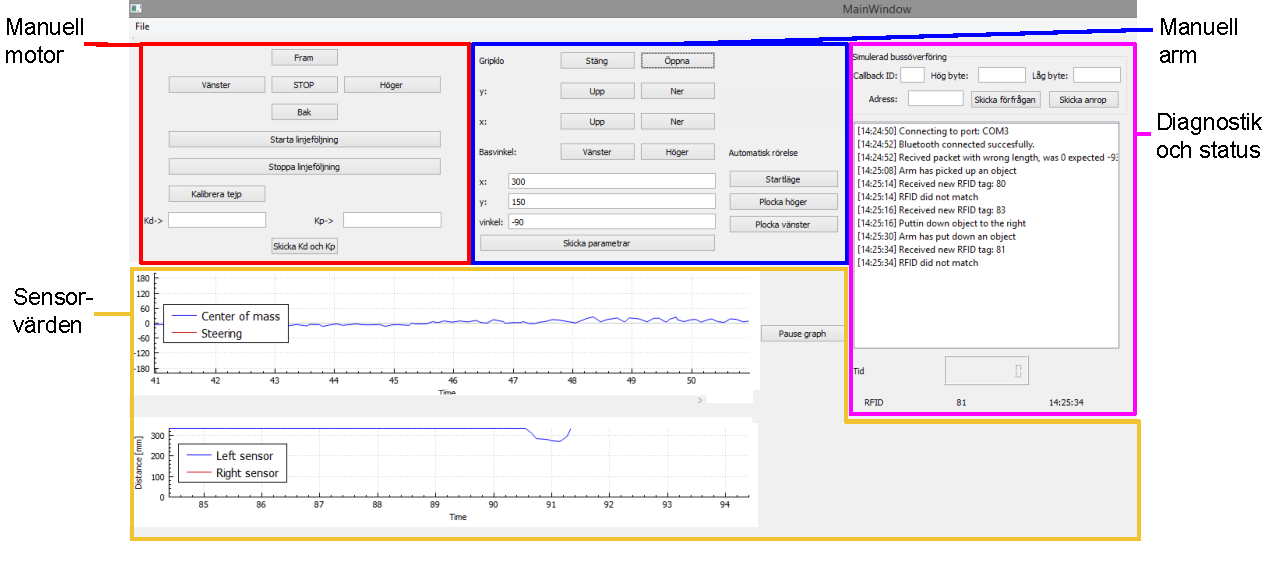
\includegraphics[width=1.0\textwidth]{PC_manual.pdf}
	\caption{Översiktlig bild av datorgränssnittet och dess olika delar}
	\label{fig:pc_oversikt}
\end{figure}

Vid manuellt läge kan användaren via PC-gränssnittet styra roboten efter behag. I automatiskt läge kan användaren använda PC-gränssnittet för att observera besluten som roboten tar och information om sensorvärden. Nedan finns en beskrivning över vad programvaran kan användas till vid manuell och automatiskt läge. 

\subsection{Motorstyrning}
\label{subsec:motor}
Säkerställ först att roboten är uppkopplad till PC via blåtand innan användning. Figur \ref{fig:pc_motor} visar instrumentbrädet för motorstyrning och tabell \ref{tab:motor} dess funktionallitet.

\begin{figure}[H]
	\centering
	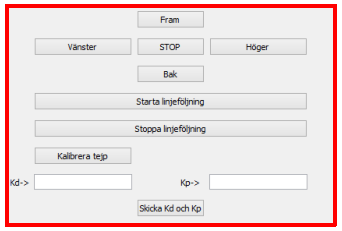
\includegraphics[width=0.6\textwidth]{man_motor1.pdf}
	\caption{Grafik över instrumentbräde för manuell styrning av roboten}
	\label{fig:pc_motor}
\end{figure}

\begin{table}[H]
\centering
\begin{tabularx}{\textwidth}{|l|X|}
\hline \textbf{Knapp / textfält} & \textbf{Funktion} \\ \hline
Fram & Ökar alla hjulens hastighet frammåt för varje användning. \\ \hline
Bak & Ökar alla hjulens hastighet bakåt för varje användning. \\ \hline
Vänster & Ökar hastighet hos höger hjulpar och minskar hastighet hos vänster hjulpar så att roboten svänger vänster, alternativt roterar. \\ \hline
Höger & Ökar hastighet hos vänster hjulpar och minskar hastighet hos höger hjulpar så att roboten svänger vänster, alternativt roterar. \\ \hline
STOP & Stannar alla hjulen. \\ \hline
Starta linjeföljning & Roboten börjar följa linje automatiskt. \\ \hline
Stoppa linjeföljning & Roboten slutar följa linje automatiskt. \\ \hline
Kalibrera tejp & Används för att kalibrera linjesensorerna så att de vet skillnad på golvet och markerad linje. Går endast när roboten står på linjen. \\ \hline
Kd & Skriv in storleken på linjeföljningsreglerarens deriverande beroende. \\ \hline
Kp & Skriv in storleken på linjeföljningsreglerarens proportionella beroende. \\ \hline
Send Kp and Kd & Skickar de värden som skrivits in i textfältet vid Kd och Kp till robototen som börjar reglera efter dessa. \\ \hline

\end{tabularx}
\caption{Tabell över funktionallitet hos manuella motorstyrningens instrumentbräde}
\label{tab:motor}
\end{table}

\subsection{Armrörelse}
Säkerställ först att roboten är uppkopplad till PC via blåtand innan användning. Nedan visas i figur \ref{fig:pc_arm} ett intrumentbräde för armrörelse samt i tabell \ref{tab:arm} dess funktionallitet.

\begin{figure}[H]
	\centering
	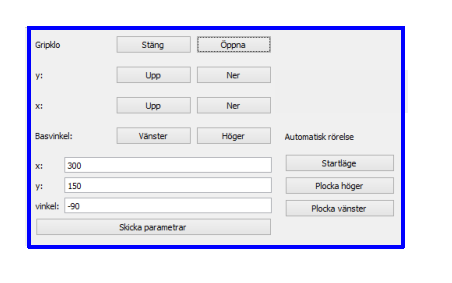
\includegraphics[width=0.6\textwidth]{armrorelse.pdf}
	\caption{Grafik över instrumentbräde för styrning av robotens arm}
	\label{fig:pc_arm}
\end{figure}

\begin{table}[H]
    \centering
    \begin{tabularx}{\textwidth}{|l|X|}
        \hline \textbf{Knapp / textfält} & \textbf{Funktion} \\ \hline
        Gripklo: Stäng& Stänger gripklo tills dess att den har stadigt grepp om föremålet eller tills maximal stängning nåtts. \\ \hline
        Gripklo: Öppna& Öppnar gripklon till maximal öppning. \\ \hline
        y: Upp & Rör armen uppåt i y-led, se figur \ref{fig:arm_koord}, så länge knappen hålls inne. \\ \hline
        y: Ner & Rör armen nedåt i y-led, se figur \ref{fig:arm_koord}, så länge knappen hålls inne. \\ \hline
        x: Upp & Rör armen uppåt i x-led, se figur \ref{fig:arm_koord}, så länge knappen hålls inne. \\ \hline
        x: Ner & Rör armen nedåt i x-led, se figur \ref{fig:arm_koord}, så länge knappen hålls inne \\ \hline
        Basvinkel: Vänster & Roterar armens bas åt vänster. \\ \hline
        Basvinkel: Höger & Roterar armens bas åt höger. \\ \hline
        x: Textfält & Här skrivs den x-koordinat, se figur \ref{fig:arm_koord}, som man vill att armen ska röra sig till i millimeter från armbasens mitt. \\ \hline
        y: Textfält & Här skrivs den y-koordinat, se figur \ref{fig:arm_koord}, som man vill att armen ska röra sig till i millimeter från armbasens mitt. \\ \hline
        vinkel: Textfält & Här skrivs den vinkel, se figur \ref{fig:arm_koord}, som man vill att armbasen ska rotera i grader. \\ \hline
        Skicka parametrar & Skickar de givna värdena x-koordinat, y-koordinat och vinkel till roboten för att utföra rörelse. \\ \hline
        Startläge & Rör automatiskt armen tillbaka till dess startläge. \\ \hline
        Plocka höger & Påbörjar skanning av område till höger för att vid identifiering av föremål sedan automatiskt plocka upp det med armen. \\ \hline
        Plocka vänster & Påbörjar skanning av område till vänster för att vid identifiering av föremål sedan automatiskt plocka upp det med armen. \\ \hline
    \end{tabularx}
\caption{Tabell över funktionallitet hos manuella motorstyrningens instrumentbräde}
\label{tab:arm}
\end{table}

\begin{figure}[H]
	\centering
	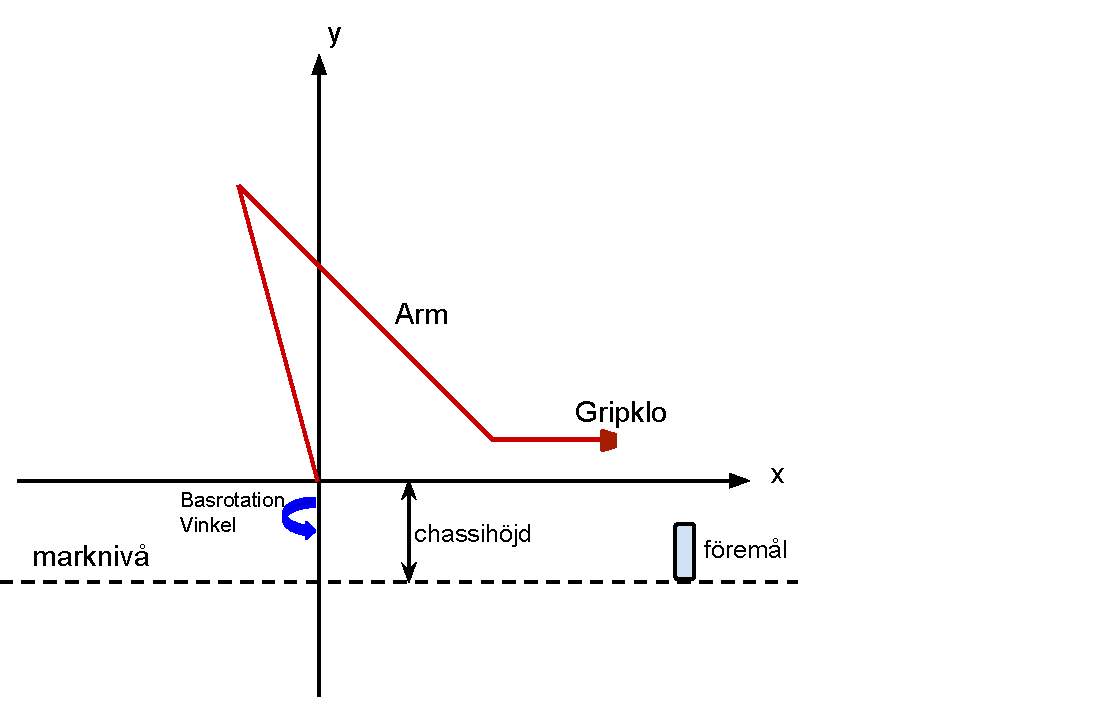
\includegraphics[width=0.6\textwidth]{arm_koord.pdf}
	\caption{Grafik över armens koordinatsystem}
	\label{fig:arm_koord}
\end{figure}

\subsection{Diagnos och status}
\label{subsec:diag}
Nedan visas i figur \ref{fig:pc_diag} ett intrumentbräde för diagnostik och status samt i tabell \ref{tab:diag} dess funktionallitet.

\begin{figure}[H]
	\centering
	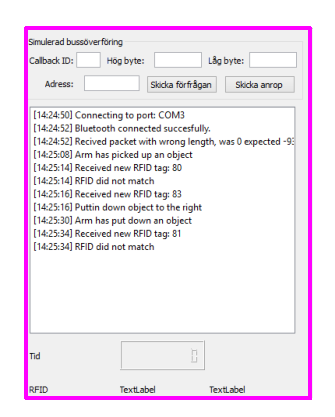
\includegraphics[width=0.6\textwidth]{diag.pdf}
	\caption{Grafik över instrumentbräde för diagnostik och status}
	\label{fig:pc_diag}
\end{figure}

\begin{table}[H]
    \centering
    \begin{tabularx}{\textwidth}{|l|X|}
        \hline \textbf{Knapp / textfält} & \textbf{Funktion} \\ \hline
        Callback ID & Bestämmer vilken funktion hos enheten du vill anropa. Se den tekniska dokumentationen, avsnitt XX för en tabell över callback-id:n \\ \hline
        Hög byte & Den mest signifikanta byten som ska skickas med anropet. Endast de tre lägsta bitarna används, totalt kan alltså 11 bitar skickas med. \\ \hline
        Låg byte & Den minst signifikanta byten som ska skickas med anropet. \\ \hline
        Adress & Bestämmer vilken enhet du vill skicka anrop till. \\ \hline
        Skicka förfrågan & Skickar en förfrågan enligt valda parametrar ovan. \\ \hline
        Skicka anrop & Utför en överföring enligt valda parametrar ovan. \\ \hline
        Loggfönster & Visar händelser som roboten observerar, status och de beslut roboten tar. Den visar också eventuella felmeddelande. Se RUBRIK XX LOGGFÖNSTER.\\ \hline
        Tid & Visar hur lång tid roboten har varit i automatiskt linjeföljningsläge. \\ \hline
    \end{tabularx}
\caption{Tabell över funktionallitet hos instrumentbrädet för diagnostik och status}
\label{tab:diag}
\end{table}

\subsection{Sensorvärden}
\label{subsec:sensor}
I figur \ref{fig:pc_sensor} visas den grafiska representationen av sensorvärden i användargränssnittet och i tabell \ref{tab:sensor} dess tolkning.

\begin{figure}[H]
	\centering
	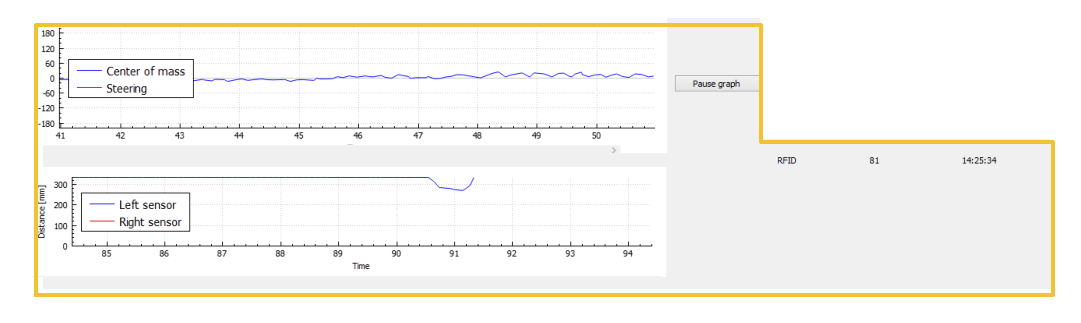
\includegraphics[width=1.0\textwidth]{sensor.pdf}
	\caption{Grafik över sensorvärdenas grafiska representation}
	\label{fig:pc_sensor}
\end{figure}

\begin{table}[H]
    \centering
    \begin{tabularx}{\textwidth}{|l|X|}
        \hline \textbf{Representation} & \textbf{Tolkning} \\ \hline
        Övre graf: blå linje & Här kan man se hur tyngdpunkten för linjesensorn förändras med tiden. Är endast på då linjeföljning är igång.\\ \hline
        Övre graf: röd linje & Här kan man se hur mycket roboten svänger höger och vänster. Roboten svänger höger då styrningen är positivt och vänster då styrningen är negativ.\\ \hline
        Undre graf: blå linje & Visar vilket avstånd som detekteras av vänster sidoskanner. Är endast igång då avsökning efter objekt sker på vänster sida. \\ \hline
        Undre graf: röd linje & Visar vilket avstånd som detekteras av höger sidoskanner. Är endast igång då avsökning efter objekt sker på höger sida. \\ \hline
        Pause graph & Stoppar uppdatering av grafen, så att användaren kan titta tillbaka på tidigare värden.\\ \hline
        RFID & Visar vilket ID det RFID som senast identifierats hade och vid vilken tid detta gjordes. \\ \hline
    \end{tabularx}
\caption{Tabell över tolkning av sensorvärdenas grafiska representation}
\label{tab:sensor}
\end{table}

\subsection{Loggfönster}
\label{subsec:logg}
I tabell \ref{tab:logg} visas de olika meddelandena och dess tolkning.


\begin{longtable}{|p{0.4\textwidth}|p{0.6\textwidth}|}
\caption{Tabell över tolkning av meddelanden i loggfönstret}\\
    \hline
    \textbf{Meddelande} & \textbf{Tolkning} \\
    \hline
    \endfirsthead
    \multicolumn{2}{c}%
    {\tablename\ \thetable\ -- \textit{Fortsättning från föregående sida}} \\
    \hline
    \textbf{Meddelande} & \textbf{Tolkning} \\
    \hline
    \endhead
    \hline \multicolumn{2}{r}{\textit{Fortsättning på nästa sida}} \\
    \endfoot
    \hline
    \endlastfoot
        \hline \textbf{Meddelande} & \textbf{Tolkning} \\ \hline
        Station to the right & Station till höger identifierad \\ \hline
        Station to the left & Station till vänster identifierad \\ \hline
        Putting down object to the right & Roboten lägger ner objekt automatiskt till höger\\ \hline
        Putting down object to the left & Roboten lägger ner objekt automatiskt till vänster \\ \hline
        ID did not match object & Det ID senaste stationen som besökts hade inte samma ID som där roboten plockat upp objekt \\ \hline
        Station is already handeld & Senaste station som identifierats har redan blivit behandlat\\ \hline
        No ID was found & Roboten hittade inte RFID-tagg på station \\ \hline
        Arm has picked up an object & Armen har automatiskt lyckats plockat upp ett objekt\\ \hline
        Arm has put down the object & Armen har automatiskt lyckats sätta ner objekt på station \\ \hline
        Object was not found by arm & Objekt har hittats på stationen \\ \hline
        An unkown error has occured & Okänt fel \\ \hline
        Arm failed pickup & Armen misslyckades att plocka upp objekt \\ \hline
        Started linefollowing & Automatisk linjeföljning startades \\ \hline
        Recived packet with wrong length, was (length 1) expected (length 2). & Packet mottaget med fel längd. \\ \hline
        Wrong checksum, was X expected Y & Packet mottaget med fel cheksum \\ \hline
        Received new RFID tag:  &  Ny RFID-tagg \\ \hline
        Calibration, new tape reference:  & Kalibrering gjord, nytt värde visas på skärmen \\ \hline
        An I/O error occurred while writing data to port 1, error: 2 & Fel vid skrivning till robot\\ \hline
        An I/O error ocurred while reading data from port 1,error:2 & Fel vid läsning från robot\\ \hline
        Device was not found. & Enheten som programmet försökte ansluta till hittades inte. \\ \hline
        Permission denied. & Tillstånd att ansluta till roboten nekat. \\ \hline
        Error while opening already openden device. & Kommunikation till roboten redan ansluten. \\ \hline
        Unknown error. & Okänt fel.\\ \hline
        Connecting to port: 1 & Ansluter till port: \\ \hline
        Bluetooth connected succesfully. & Lyckades ansluta till roboten. \\ \hline
        Error opening bluetooth & Fel vid försök att ansluta till roboten.\\ \hline
        No port to send to. & Ingen enhet ansluten via blåtand. \\ \hline
        Sent arm command & Arm kommando skickat. \\ \hline
        x: 1, y: 2, angle: 3 & Parametrar som skickades till armen. \\ \hline
        Invalid arguments to arm position, must be integers. & Inskriven position var inte tal. \\ \hline
        Station left:  & Station till vänster. \\ \hline
        Station right & Station till höger. \\ \hline
        Break in line. & Avbrott i linjen.
\label{tab:logg}
\end{longtable}


\newpage
\section*{Referenser}


\newpage
\appendix

\end{document} 
